\documentclass[12pt]{article}
\usepackage[utf8]{inputenc}
\usepackage{lmodern}
\usepackage[T1]{fontenc}
\usepackage{amsmath}
\usepackage{enumitem}
\usepackage{graphicx}
\usepackage{fullpage}
\usepackage{siunitx}
\usepackage{fancyhdr}
\PassOptionsToPackage{hyphens}{url}
\usepackage[hyphens]{url}
\usepackage{color}
\usepackage{enumitem}
\usepackage{textcomp}
\usepackage{geometry}
\usepackage{courier}
\usepackage{listings}
\usepackage{array}
\usepackage{amsthm}
\usepackage{mathdots}
\usepackage{amssymb}
\usepackage{minted}
\usepackage{wrapfig}
\usepackage{titlesec}
\usepackage{parskip}
\usepackage{accents}
\usepackage{gensymb}
\usepackage{indentfirst}
\usepackage{courier}
\usepackage{framed}
\usepackage{etoolbox}
\usepackage{titlesec}
\usepackage{appendix}
\usepackage{mdframed}
\usepackage{verbatim}
\usepackage{xspace}
\usepackage{hyperref}
\usepackage[utf8]{inputenc}
\usepackage{quotchap}

\AtBeginEnvironment{subappendices}{%
	\section*{Appendix}
	\addcontentsline{toc}{section}{Appendices}
}

%\lstset{language=C++,
%                basicstyle=\ttfamily,
%                keywordstyle=\color{blue}\ttfamily,
%                stringstyle=\color{red}\ttfamily,
%                commentstyle=\color{green}\ttfamily,
%                morecomment=[l][\color{magenta}]{\#}
%}

\definecolor{keywordcolor}{rgb}{0,0,0.45}
\definecolor{stringcolor}{rgb}{0.45,0.45,0.45}
\definecolor{commentcolor}{rgb}{0,0.3,0}

\lstset{
	language=C++,
	basicstyle=\footnotesize\ttfamily,
	numbers=left,
	%numberstyle=\tiny,
	frame=tb,
	columns=fullflexible,
	showstringspaces=false,
	breaklines=true,
	tabsize=4,
	keywordstyle=\color{keywordcolor}\footnotesize\bf\ttfamily,
	stringstyle=\color{stringcolor}\footnotesize\ttfamily,
	commentstyle=\color{commentcolor}\it\sffamily
}
% \lstset{basicstyle=\ttfamily,breaklines=true}
\lstloadlanguages{C++}

%\renewcommand{\familydefault}{\sfdefault}

\addtolength{\parskip}{\baselineskip}  
\newcommand{\urlwofont}[1]{\urlstyle{same}\url{#1}}

\renewcommand{\arraystretch}{0.8}
\renewcommand{\headrulewidth}{0pt}
\renewcommand{\footrulewidth}{0pt}

\newcommand{\imagewidth}{0.8\textwidth}

\lhead{}
\chead{}
\rhead{}
\lfoot{}
\cfoot{\thepage}
\rfoot{}

\geometry{
	top=0.9in,
	inner=0.7in,
	outer=0.7in,
	bottom=0.9in,
	headheight=2ex,
	headsep=1ex,
}
\pagestyle{fancy}
%\fancyhf{}
%\setlength{\headsep}{0.2in}


\fancypagestyle{firststyle}
{
	\chead{}
	\setlength{\headsep}{0.0in}
}
\hypersetup{
	unicode=true,
	colorlinks=true,
	linkcolor=blue,
	citecolor=black,
	filecolor=black,
	urlcolor=blue
}

\begingroup
\makeatletter
\@for\theoremstyle:=definition,remark,plain\do{%
	\expandafter\g@addto@macro\csname th@\theoremstyle\endcsname{%
		\addtolength\thm@preskip\parskip
	}%
}
\endgroup

\newtheorem{thm}{Theorem}[section]
\newtheorem{lemma}{Lemma}[section]
\newtheorem{claim}{Claim}[section]
\newtheorem{proposition}{Proposition}[section]
%\theoremstyle{empty}
\newtheorem*{namedthm}{Theorem}

% indention size
%\setlength{\parindent}{19pt}
\setlength{\parindent}{0pt}

% paragraph spacing
\setlength{\parskip}{1em}

% line spacing
\linespread{1}

%\setcounter{tocdepth}{1}


% Documenting starts here! Please do not change above! 

\newcommand{\mytitle}
{
	\textbf {
		inzva Algorithm Programme 2018-2019\\ \ \\
		Bundle 5 \\ \ \\ 
		DP - 1 \\ \ \\
	}
}

\title{\vspace{-2em}\mytitle\vspace{-0.3em}}

\author{
	\textbf{Editor}\\
	Halil Çetiner  \\ \ \\ 
	\textbf{Reviewer(s)} \\ 
	Onur Yıldız
}

\date{}
\begin{document}
	
	\begin{figure}
		\centering
		
\includegraphics[width=\linewidth/4]{inzva-logo.png}
		\label{fig:inzva}
	\end{figure}
	\maketitle
	
	\cleardoublepage
	\tableofcontents
	\markboth{Table of Contents}{}
	\cleardoublepage
	\section{Greedy Algorithms}
	A \textbf{greedy algorithm} is an algorithm that follows the problem solving heuristic of making the locally optimal choice at each stage with the hope of finding a global optimum. A greedy algorithm never takes back its choices, but directly constructs the final solution. For this reason, greedy algorithms are usually very efficient.\\
    The difficulty in designing greedy algorithms is to find a greedy strategy that always produces an optimal solution to the problem. The locally optimal choices in a greedy algorithm should also be globally optimal. It is often difficult to argue that a greedy algorithm works.
	\subsection{Coin Problem}
	We are given a value V, if we want to make change for V cents, and we have an infinite supply of each of the coins = \{ C1, C2, .. , Cm \} valued coins (sorted in descending order), what is the minimum number of coins to make the change?
	\subsubsection{Solution}
    Approach:
	\begin{lstlisting}[numbers=none, frame=none]
1- Initialize the result as empty.
2- Find the largest denomination that is 
smaller than amount.
3- Add found denomination to the result. Subtract 
the value of found denomination from amount.
4 - If amount becomes 0, then print the result.  
Else repeat the steps 2 and 3 for the new value of amount
	\end{lstlisting}
	
	For example, if the coins are the euro coins (in cents) {200,100,50,20,10,5,2,1} and the amount is 548.\\
	Then the optimal solution is to select coins 200+200+100+20+20+5+2+1 whose sum is 548.
	\begin{figure}[h!]
        	\centering
        	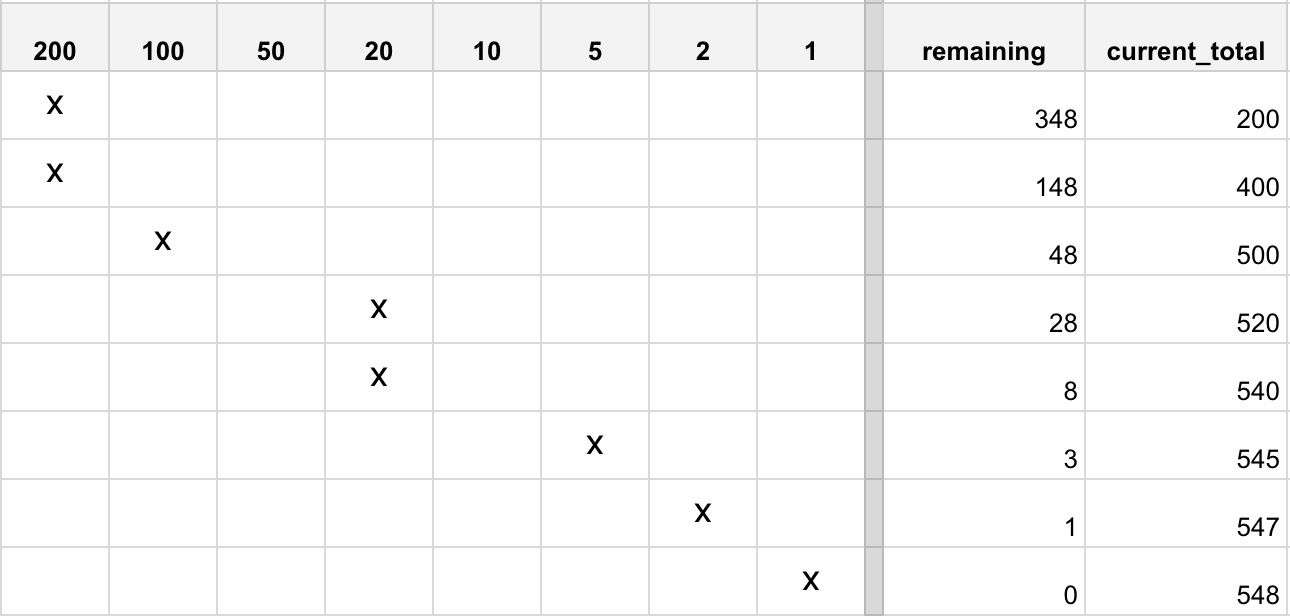
\includegraphics[width=.7\linewidth]{template/coin_greedy.png}
        	\label{fig:coin_greedy}
        \end{figure}
	
	\begin{lstlisting}[language=Python]
	def min_coins(coins, amount):
	    n = len(coins)
        for (i in range(0, n)):
        while (amount >= coins[i]):
            #while loop is needed since one coin can be used multiple times
            amount = amount - coins[i]
            print(coins[i])

    \end{lstlisting}
    In the general case, the coin set can contain any kind of coins and the greedy algorithm does not necessarily produce an optimal solution.\\
    We can prove that a greedy algorithm does not work by showing a counterexample where the algorithm gives a wrong answer.\\
    In this problem we can easily find a counterexample: if the coins are {6,5,2} and the target sum is 10, the greedy algorithm produces the solution 6+2+2 while the optimal solution is 5+5.
    \subsection{Scheduling}
    Many scheduling problems can be solved using greedy algorithms. A classic problem is as follows:\\
    We are given an array of jobs where every job has a deadline and associated profit if the job is finished before the deadline. It is also given that every job takes single unit of time, thus the minimum possible deadline for any job is 1. How do we maximize total profit if only one job can be scheduled at a time.
    \subsubsection{Solution}
    A Simple Solution is to generate all subsets of the given set of jobs and check an individual subset for the feasibility of jobs in that subset. Keep track of maximum profit among all feasible subsets. The time complexity of this solution is exponential.
    This is a standard Greedy Algorithm problem. Following is the algorithm:
	\begin{lstlisting}[numbers=none, frame=none]
1- Sort all jobs in decreasing order of profit.
2- Initialize the result sequence as the first job in sorted jobs.
3- Do the following for the remaining n-1 jobs
        If the current job can fit in the current result sequence without missing the deadline, add the current job to the result.
        Else ignore the current job.
	\end{lstlisting}
	
	\begin{lstlisting}[language=Python]
	# sample job : ['x', 4, 25] -> [job_id, deadline, profit]
	# jobs: array of 'job's
	def print_job_scheduling(jobs, t): 
        n = len(jobs) 
        
        # Sort all jobs according to decreasing order of profit 
        for (i in range(n)): 
            for (j in range(n - 1 - i)): 
                if (jobs[j][2] < jobs[j + 1][2]): 
                    jobs[j], jobs[j + 1] = jobs[j + 1], jobs[j] 
        
        # To keep track of free time slots 
        result = [False] * t 
        # To store result (Sequence of jobs) 
        job = ['-1'] * t 
        
        # Iterate through all given jobs 
        for (i in range(len(jobs))): 
        
            # Find a free slot for this job  
            # (Note that we start from the last possible slot) 
            for (j in range(min(t - 1, jobs[i][1] - 1), -1, -1)): 
                  
                # Free slot found 
                if (result[j] is False): 
                    result[j] = True
                    job[j] = jobs[i][0] 
                    break
        print(job) 

    \end{lstlisting}
    
    \subsection{Tasks and Deadlines}
    Let us now consider a problem where we are given n tasks with the durations and deadlines and our task is to choose an order to perform the tasks. For each task, we earn d \-- x points where d is the task’s deadline and x is the moment when we finish the task. What is the largest possible total score we can obtain?\\
    For example, suppose that the tasks are as follows:\\
    \[\{task, duration, deadline\}\]
    \[\{A, 4, 2\} , \{B, 3, 5\} , \{C, 2, 7\} , \{D, 4, 5\}\]
    
    In this case, an optimal schedule for the tasks is C, B, A, D.\\
    In this solution, C yields 5 points, B yields 0 points, A yields \--7 points and D yields \--8 points, so the total score is \--10.\\
    Surprisingly, the optimal solution to the problem does not depend on the deadlines at all, but a correct greedy strategy is to simply perform the tasks sorted by their durations in increasing order. The reason for this is that if we ever perform two tasks one after another such that the first task takes longer than the second task, we can obtain a better solution if we swap the tasks.
    \newpage
    \subsubsection{Solution}
     \begin{lstlisting}[language=Python]
     def order_tasks(task):
        n = len(tasks) 
        
        # Sort all task according to increasing order of duration 
        for (i in range(n)): 
            for (j in range(n - 1 - i)): 
                if (tasks[j][1] > tasks[j + 1][1]): 
                    tasks[j], tasks[j + 1] = tasks[j + 1], tasks[j]
        
        point = 0
        current_time = 0
        # Iterate through all given tasks and calculate point
        for (i in range(len(tasks))): 
            current_time = current_time + tasks[i][1]
            point = point + (tasks[i][2] - current_time)
            
        print(point) 
        
    \end{lstlisting}
    \subsection{Minimizing Sums}
    Where we are given n numbers and our task is to find a value x that minimizes the sum:
    \[|a_1 \-- x|\textsuperscript{c} +|a_2 \-- x|\textsuperscript{c} + ... +|a_n \-- x|\textsuperscript{c}.\]
    We focus on the cases c = 1 and c = 2.
    
    \textbf{• Case c = 1}\\
    In this case, we should minimize the sum
    \[|a_1 \-- x| +|a_2 \-- x| + ... +|a_n \-- x|\]
    For example, if the numbers are [1,2,9,2,6], the best solution is to select x = 2 which produces the sum
    \[|1\--2| +|2\--2| +|9\--2| +|2\--2| +|6\--2| = 12.\]
    In the general case, the best choice for x is the median of the numbers, i.e., the middle number after sorting. For example, the list [1,2,9,2,6] becomes [1,2,2,6,9] after sorting, so the median is 2.\\
    The median is an optimal choice, because if x is smaller than the median, the sum becomes smaller by increasing x, and if x is larger then the median, the sum becomes smaller by decreasing x. Hence, the optimal solution is that x is the median. If n is even and there are two medians, both medians and all values between them are optimal choices.
    
    \textbf{• Case c = 2}\\
    In this case, we should minimize the sum:
    \[(a_1 \-- x)\textsuperscript{2} + (a_2 \-- x)\textsuperscript{2} + ... + (a_n \-- x)\textsuperscript{2}.\]
    For example, if the numbers are [1,2,9,2,6], the best solution is to select x = 4 which produces the sum:
    \[(1\-- 4)\textsuperscript{2} + (2\-- 4)\textsuperscript{2} +(9\-- 4)\textsuperscript{2} + (2\--4)\textsuperscript{2} + (6\--4)\textsuperscript{2} = 46\]
    
    In the general case, the best choice for x is the average of the numbers. In the example the average is (1 + 2 + 9 + 2 + 6)/5 = 4.\\
    This result can be derived by presenting the sum as follows:
    \[nx\textsuperscript{2} \-- 2x(a_1 + a_2 + ... + a_n) + (a_1\textsuperscript{2} + a_2\textsuperscript{2} + ... + a_n\textsuperscript{2})\]
    
    The last part does not depend on x, so we can ignore it. The remaining parts form a function 
    \[nx\textsuperscript{2} − 2xs\]
    \[s = a_1 + a_2 + ... + a_n.\]
    
    This is a parabola opening upwards with roots x = 0 and x = 2s/n, and the minimum value is the average of the roots x = s/n, i.e., the average of the numbers.
    \newpage
	\section{Dynamic Programming}
	\textbf{Dynamic programming} is a technique used to avoid computing multiple times the same sub-solution in a recursive algorithm. A sub-solution of the problem is constructed from the previously found ones. DP solutions have a polynomial complexity which assures a much faster running time than other techniques like backtracking, brute-force etc.
	
	\subsection{Memoization - Top Down}
	Memoization ensures that a method doesn't run for the same inputs more than once by keeping a record of the results for the given inputs (usually in a hash map).
	
	To avoid the duplicate work caused by the branching, we can wrap the method in a class that stores an instance variable, cache, that maps inputs to outputs. Then we simply,
    \begin{itemize}
        \item check cache to see if we can avoid computing the answer for any given input, and
        \item save the results of any calculations to cache.
    \end{itemize}
    
    Memoization is a common strategy for dynamic programming problems, which are problems where the solution is composed of solutions to the same problem with smaller inputs (as with the Fibonacci problem, above). \\The other common strategy for dynamic programming problems is going bottom-up, which is usually cleaner and often more efficient.
    	
	\subsection{Bottom Up}
	Going bottom-up is a way to avoid recursion, saving the memory cost that recursion incurs when it builds up the call stack.\\

    Simply a bottom-up algorithm "starts from the beginning," while a recursive algorithm often "starts from the end and works backwards."
	
	\subsection{An example - Fibonacci}
	Let's start with an example which most of us are familiar, fibonacci numbers: finding the n\textsuperscript{th} fibonacci number defined by\\
    \begin{align*}
    F_n = F_{n-1} + F_{n-2} \quad \textrm{and} \quad F_0 = 0,   F_1 = 1
    \end{align*}
    
    There are a few approaches and all of them work. Let's go through the codes and see the cons and pros:
	\subsubsection{Recursion}
	
    \begin{lstlisting}[language=Python]
    def fibonacci(n):
        if (n == 0):
            return 0
        if (n == 1):
            return 1
    
        return fibonacci(n - 1) + fibonacci(n - 2)
    \end{lstlisting}

	\subsubsection{Dynamic Programming}
        
	\begin{itemize}
		\item \textbf{Top Down - Memoization} \\\\ The recursion does a lot of unnecessary calculation because a given fibonacci number will be calculated multiple times. An easy way to improve this is to cache the results (memoization):
		
		\begin{lstlisting}[language=Python]
        cache = {}

        def fibonacci(n):
            if (n == 0):
                return 0
            if (n == 1):
                return 1
            if (n in cache):
                return cache[n]
        
            cache[n] = fibonacci(n - 1) + fibonacci(n - 2)
        
            return cache[n]
        \end{lstlisting}
        
	\begin{figure}[h!]
        	\centering
        	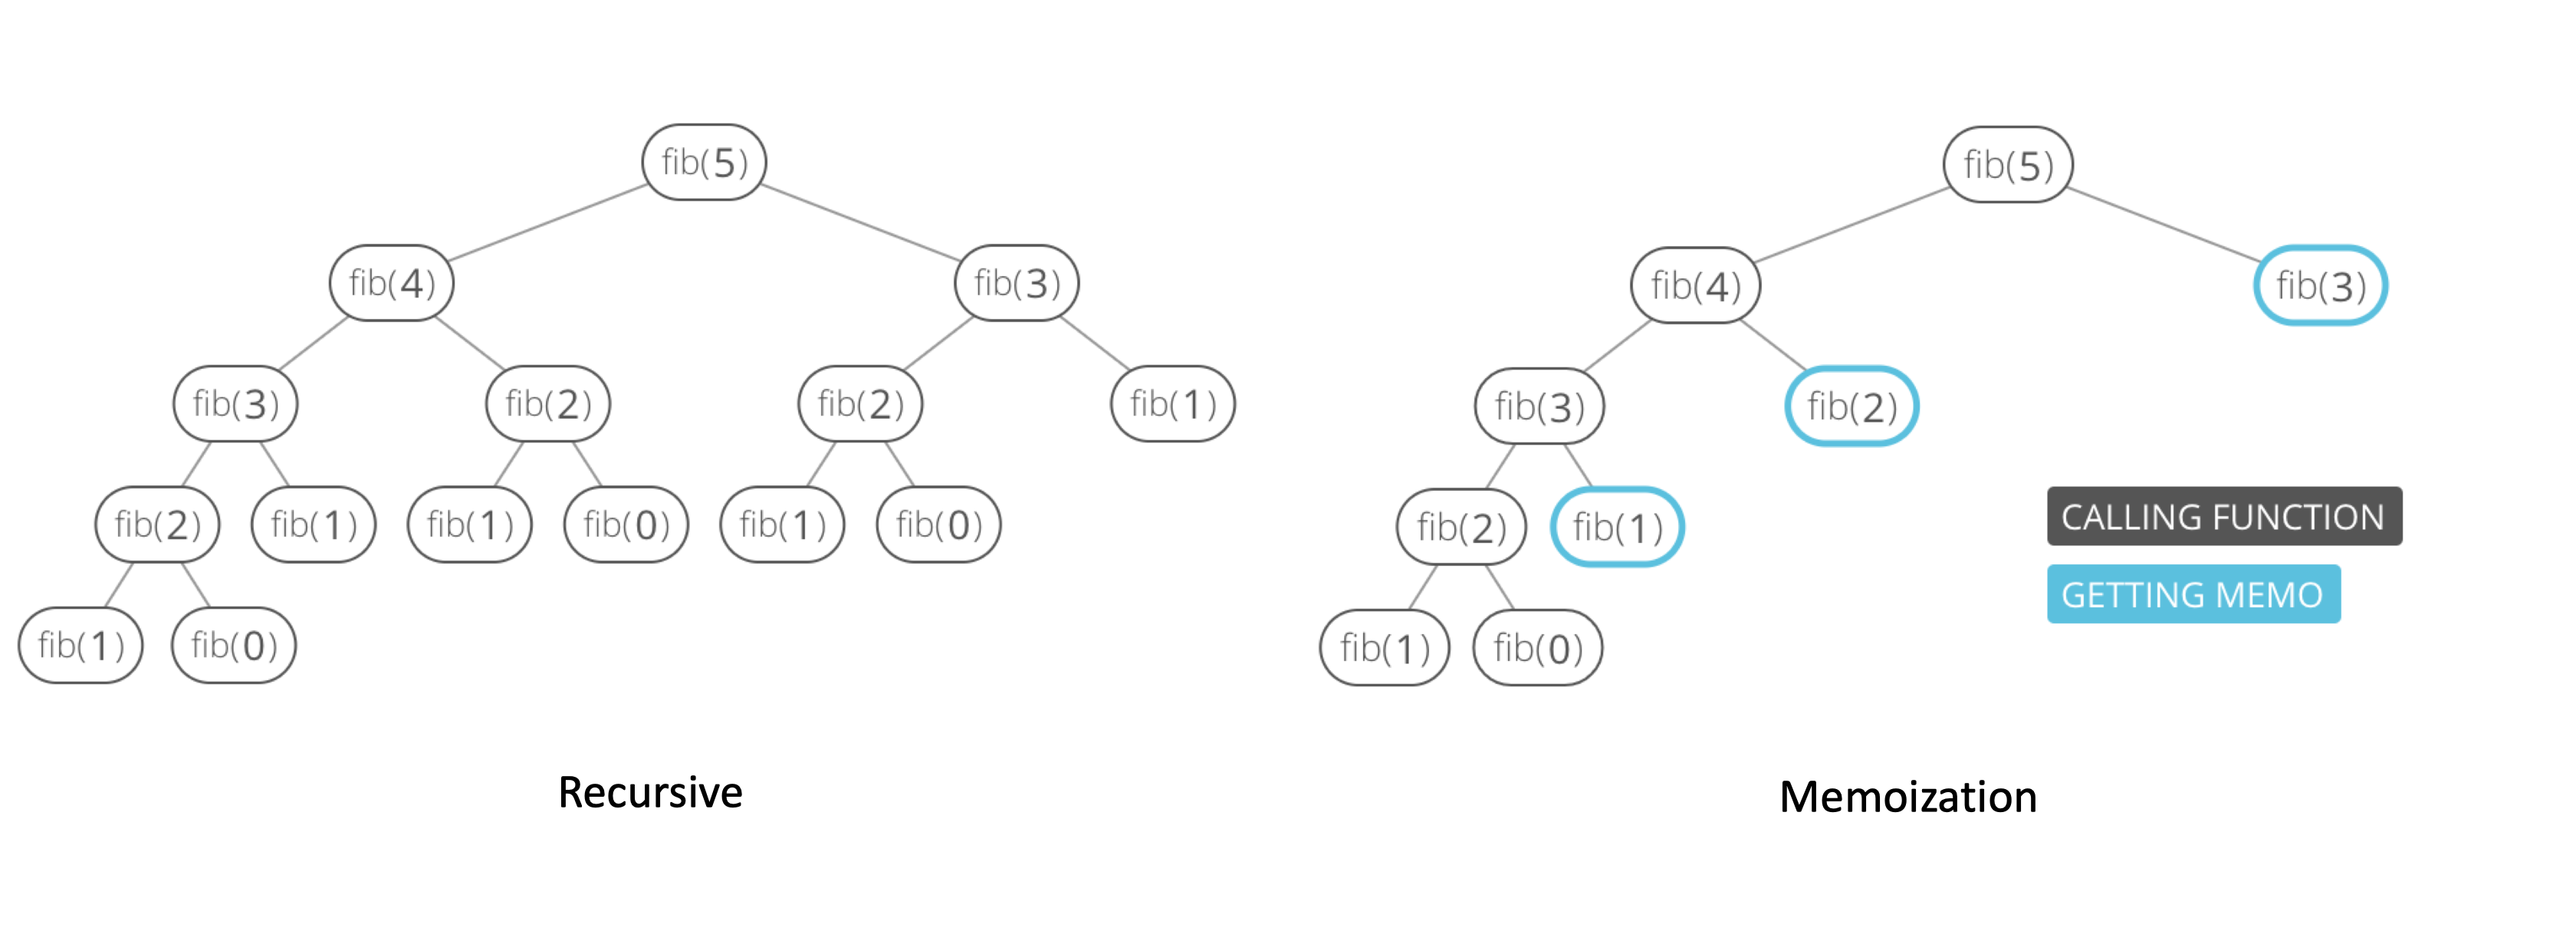
\includegraphics[width=.8\linewidth]{template/rec_vs_mem.png}
        	\label{fig:recursive_vs_memoization}
        \end{figure}
        
        
		\item \textbf{Bottom-Up} \\\\ A better way to do this is to get rid of the recursion all-together by evaluating the results in the right order:
		
		\begin{lstlisting}[language=Python]
        cache = {}

        def fibonacci(n):
            cache[0] = 0
            cache[1] = 1
        
            for (i in range(2, n + 1)):
                cache[i] = cache[i - 1] +  cache[i - 2]
        
            return cache[n]
        \end{lstlisting}
        We can even use constant space, and store only the necessary partial results along the way:
        
		\begin{lstlisting}[language=Python]
        def fibonacci(n):
          fib_minus_2 = 0
          fib_minus_1 = 1
        
          for (i in range(2, n + 1)):
              fib = fib_minus_1 + fib_minus_2
              fib_minus_1, fib_minus_2 = fib, fib_minus_1
        
          return fib
        \end{lstlisting}
		
	\end{itemize}
	
	\subsection{How to Apply Dynamic Programming?}
		\begin{itemize}
    		\item {Find the recursion in the problem.}
    		\item {\textbf{Top-down:} store the answer for each subproblem in a table to avoid having to recompute them.}
		    \item {\textbf{Bottom-up:} Find the right order to evaluate the results so that partial results are available when needed.}
		\end{itemize}
		Dynamic programming generally works for problems that have an inherent left to right order such as strings, trees or integer sequences. If the naive recursive algorithm does not compute the same subproblem multiple time, dynamic programming won't help.
    
	
	\newpage
	\section{Common DP Problems}
	\subsection{Coin Problem}
	As we discussed above Greedy approach doesn't work all the time for the coin problem. \\
	For example: if the coins are {4,3,1} and the target sum is 6, the greedy algorithm produces the solution 4+1+1 while the optimal solution is 3+3.\\
	This is where Dynamic Programming helps us:
	\subsubsection{Solution}
    Approach:
	\begin{lstlisting}[numbers=none, frame=none]
    1- If V == 0, then 0 coins required.
    2- If V > 0,   minCoins(coins[0..m-1], V) = min {1 + minCoins(V-coin[i])}
                  where i varies from 0 to m-1
                  and coins[i] <= V
	\end{lstlisting}
	
	\begin{lstlisting}[language=Python]
	def minCoins(coins, target): 
        # base case 
        if (V == 0): 
            return 0
        
	    n = len(coins) 
        # Initialize result 
        res = sys.maxsize 
          
        # Try every coin that has smaller value than V 
        for i in range(0, n): 
            if (coins[i] <= target): 
                sub_res = minCoins(coins, target-coins[i]) 
      
                # Check for INT_MAX to avoid overflow and see if 
                # result can minimized 
                if (sub_res != sys.maxsize and sub_res + 1 < res): 
                    res = sub_res + 1
      
        return res 
        
    \end{lstlisting}
	\newpage
	\subsection{Knapsack Problem}
	We are given the weights and values of n items, put these items in a knapsack of capacity W to get the maximum total value in the knapsack. In other words, given two integer arrays val[0..n-1] and wt[0..n-1] which represent the values and weights associated with n items respectively. Also given an integer W which represents knapsack capacity, find out the maximum value subset of val[] such that sum of the weights of this subset is smaller than or equal to W. You cannot break an item, either pick the complete item; or don’t pick it (0-1 property).\\
    Approach:
	\begin{lstlisting}[numbers=none, frame=none]
To consider all subsets of items, there can be two cases for every item: (1) the item is included in the optimal subset, (2) not included in the optimal set.

Therefore, the maximum value that can be obtained from n items is max of the following two values.
1- Maximum value obtained by n-1 items and W weight (excluding nth item).
2- Value of the nth item plus the maximum value obtained by n-1 items and W minus the weight of the nth item (including the nth item).

If the weight of nth item is greater than W, then the nth item cannot be included and case 1 is the only possibility.
   
	\end{lstlisting}
	
	For example:
	\begin{lstlisting}[numbers=none, frame=none]
	Let,
	Knapsack Max weight: W = 8 (units)
    Weight of items:  wt = {3, 1, 4, 5}
    Values of items: val = {10, 40, 30, 50}
    Total items: n = 4
    
    Then,
    The following sums are possible:
    1, 3, 4, 5, 6, 7, 8, 9, 10, 12, 13
    
    The sum 8 is possible with 2 combinations
    {3, 5} and  {1, 3, 4}
    
    for {3, 5} total value is 60
    and for {1, 3, 4} total value is 80
    
    Hence,
    Our answer for maximum total value in the knapsack with given items and knapsack will be 80.
    \end{lstlisting}
    \newpage
	\subsubsection{Recursion}
	\begin{lstlisting}[language=Python]
	def knapSack(W , wt , val , n): 
  
        # Base Case 
        if (n == 0 or W == 0): 
            return 0
      
        # If weight of the nth item is more than Knapsack of capacity 
        # W, then this item cannot be included in the optimal solution 
        if (wt[n-1] > W): 
            return knapSack(W , wt , val , n - 1) 
      
        # return the maximum of two cases: 
        # (1) nth item included 
        # (2) not included 
        else: 
            return max(val[n-1] + knapSack(W - wt[n - 1] , wt , val , n - 1), knapSack(W , wt , val , n - 1)) 
        
    \end{lstlisting}
	\subsubsection{DP}
    It should be noted that the above function computes the same subproblems again and again. Time complexity of this naive recursive solution is exponential (2\textsuperscript{n}).\\
    Since suproblems are evaluated again, this problem has Overlapping Subproblems property. Like other typical Dynamic Programming(DP) problems, recomputations of same subproblems can be avoided by constructing a temporary array K[][] in bottom up manner. Following is Dynamic Programming based implementation. 
	
	\begin{lstlisting}[language=Python]
	def knapSack(W, wt, val, n): 
        K = [[0 for x in range(W + 1)] for x in range(n + 1)] 
      
        # Build table K[][] in bottom up manner 
        for (i in range(n + 1)): 
            for (w in range(W + 1)): 
                if (i == 0 or w == 0): 
                    K[i][w] = 0
                elif (wt[i - 1] <= w): 
                    K[i][w] = max(val[i - 1] + K[i - 1][w - wt[i - 1]], K[i - 1][w]) 
                else: 
                    K[i][w] = K[i - 1][w] 
      
        return K[n][W] 
        
    \end{lstlisting}
    \newpage
	\subsection{Longest Common Substring (LCS) Problem}
	We are given two strings ‘X’ and ‘Y’, find the length of the longest common substring.\\
	Sample Case:
	\begin{lstlisting}[numbers=none, frame=none]
Input: X="inzvahackerspace", Y="spoilerspoiler"
Output: 4
The longest common substring is "ersp" and is of length 4.
	\end{lstlisting}
	
	Let m and n be the lengths of the first and second strings respectively.

    A simple solution is to one by one consider all substrings of the first string and for every substring check if it is a substring in the second string. Keep track of the maximum length substring. There will be O(m\textsuperscript{2}) substrings and we can find whether a string is subsring on another string in O(n) time (See this). So overall time complexity of this method would be O(n * m\textsuperscript{2}).

    Dynamic Programming can be used to find the longest common substring in O(m*n) time. The idea is to find the length of the longest common suffix for all substrings of both strings and store these lengths in a table.
	
	\begin{lstlisting}[numbers=none, frame=none]
The longest common suffix has following optimal substructure property
    LCSuff(X, Y, m, n) = LCSuff(X, Y, m-1, n-1) + 1
    if X[m-1] = Y[n-1] 0  Otherwise (if X[m-1] != Y[n-1])

The maximum length Longest Common Suffix is the longest common substring.
    LCSubStr(X, Y, m, n) = Max(LCSuff(X, Y, i, j)) where 1 <= i <= m and 1 <= j <= n
	\end{lstlisting}
	\newpage
	\subsubsection{DP - Iterative}
	
	\begin{lstlisting}[language=Python]
	def LCSubStr(X, Y): 
    	m = len(X) 
        n = len(Y) 
        
        # Create a table to store lengths of 
        # longest common suffixes of substrings.  
        # Note that LCSuff[i][j] contains the  
        # length of longest common suffix of  
        # X[0...i-1] and Y[0...j-1]. The first 
        # row and first column entries have no 
        # logical meaning, they are used only 
        # for simplicity of the program. 
          
        # LCSuff is the table with zero  
        # value initially in each cell 
        LCSuff = [[0 for k in range(n+1)] for l in range(m + 1)] 
          
        # To store the length of  
        # longest common substring 
        result = 0 
      
        # Following steps to build 
        # LCSuff[m+1][n+1] in bottom up fashion 
        for (i in range(m + 1)): 
            for (j in range(n + 1)): 
                if (i == 0 or j == 0): 
                    LCSuff[i][j] = 0
                elif (X[i - 1] == Y[j - 1]): 
                    LCSuff[i][j] = LCSuff[i - 1][j - 1] + 1
                    result = max(result, LCSuff[i][j]) 
                else: 
                    LCSuff[i][j] = 0
        return result 
        
    \end{lstlisting}
	\subsubsection{DP - Recursive}
	
	\begin{lstlisting}[language=Python]
	def lcs(int i, int j, int count):
        if (i == 0 or j == 0):
            return count
              
        if (X[i - 1] == Y[j - 1]):
            count = lcs(i - 1, j - 1, count + 1)
            
        count = max(count, max(lcs(i, j - 1, 0), lcs(i - 1, j, 0))) 
        return count
        
    \end{lstlisting}
	\subsection{Longest Increasing Subsequence (LIS) Problem}
	The Longest Increasing Subsequence (LIS) problem is to find the length of the longest subsequence of a given sequence such that all elements of the subsequence are sorted in theincreasing order.\\
	For example, given the array [0, 8, 4, 12, 2, 10, 6, 14, 1, 9, 5, 13, 3, 11, 7, 15], the longest increasing subsequence has the length of 6: it is \{0, 2, 6, 9, 11, 15\}.
	\subsubsection{Solution}
	The naive, brute force way to solve this is to generate each possible subsequence, testing each one for monotonicity and keeping track of the longest one. That would be prohibitively expensive: generating each subsequence already takes O(2\textsuperscript{N})!\\
    Instead, let’s try to tackle this problem using recursion and then optimize it with dynamic programming.\\
    Assume that we already have a function that gives us the length of the longest increasing subsequence. Then we’ll try to feed some part of our input array back to it and try to extend the result. Our base cases are: the empty list, returning 0, and an array with one element, returning 1.\\
    Then,
    \begin{itemize}
        \item For every index i up until the second to last element, calculate longest\_increasing\_subsequence up to there.
        \item We can only extend the result with the last element if our last element is greater than arr[i] (since otherwise it’s not increasing).
        \item Keep track of the largest result.
    \end{itemize}
    
    \begin{lstlisting}[language=Python]
	def longest_increasing_subsequence(arr):
        if (not arr):
            return 0
        if (len(arr) == 1):
            return 1
    
        max_ending_here = 0
        for (i in range(len(arr))):
            ending_at_i = longest_increasing_subsequence(arr[:i])
            if (arr[-1] > arr[i - 1] and ending_at_i + 1 > max_ending_here):
                max_ending_here = ending_at_i + 1
        return max_ending_here
        
    \end{lstlisting}
    
    This is really slow due to repeated subcomputations (exponential in time). So, let’s use dynamic programming to store values to recompute them for later.
    \newpage
    We’ll keep an array A of length N, and A[i] will contain the length of the longest increasing subsequence ending at i. We can then use the same recurrence but look it up in the array instead:
    
    
    \begin{lstlisting}[language=Python]
	def longest_increasing_subsequence(arr):
        if (not arr):
            return 0
        cache = [1] * len(arr)
        for (i in range(1, len(arr))):
            for (j in range(i)):
                if (arr[i] > arr[j]):
                    cache[i] = max(cache[i], cache[j] + 1)
        return max(cache)
        
    \end{lstlisting}
    
    This now runs in O(N\textsuperscript{2}) time and O(N) space.
	\newpage
	\section{Conclusion}
	As we discussed,\\
	Dynamic programming is a technique that combines the correctness of complete search and the efficiency of greedy algorithms. Dynamic programming can be applied if the problem can be divided into overlapping subproblems that can be solved independently.\\
	There are two uses for dynamic programming:
	\begin{itemize}
	    \item \textbf{Finding an optimal solution:} We want to find a solution that is as large
as possible or as small as possible.
        \item \textbf{Counting the number of solutions:} We want to calculate the total number of possible solutions.
	\end{itemize}
	\vfill
	
	\begin{center}
	    “Those who cannot remember the past are condemned to repeat it.” \\ George Santayana
	\end{center}
	
	\newpage
	\begin{thebibliography}{0}
		
		\bibitem{turing}
		"Competitive Programmer’s Handbook" by Antti Laaksonen - Draft July 3, 2018 \url{https://cses.fi/book/book.pdf}
		\bibitem{wiki}
		Wikipedia - Dynamic Programming
		\url{https://en.wikipedia.org/wiki/Dynamic_programming}
		\bibitem{topcoder}
		Topcoder - Competitive Programming Community / Dynamic Programming from Novice to Advanced
		\url{https://www.topcoder.com/community/competitive-programming/tutorials/dynamic-programming-from-novice-to-advanced/}
		\bibitem{hacker_earth}
		Hacker Earth - Dynamic Programming
		\url{https://www.hackerearth.com/practice/algorithms/dynamic-programming/}
		\bibitem{geeks_for_geeks}
		Geeks for Geeks - Dynamic Programming \url{https://www.geeksforgeeks.org/dynamic-programming/}
	\end{thebibliography}

\end{document}
